\lecture{1}{26. August 2025}{Introduction}

\exercise{1.1}
We consider the rotation of a rigid body shown in \textbf{\autoref{fig:e1_1}} about the point $O$. The rod has mass $m$ and the spring fastened to the rod at distance $L$ from the point $O$ has stiffness $k$. A force $F(t)$ is applied at a distance $L/2$ from the point $O$.

\begin{figure} [ht]
  \centering
  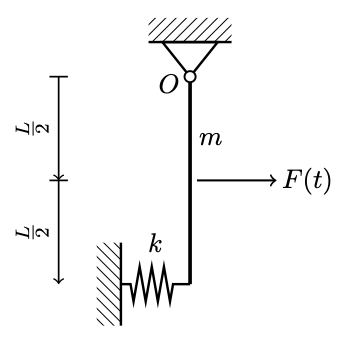
\includegraphics[width=0.35\linewidth]{./figures/e1_1.png}
  \caption{}
  \label{fig:e1_1}
\end{figure}

\paragraph{a)} Derive the non-linear equation of motion for the rotation of the rigid body.
\bigbreak
We determine the resultant moment around $O$ as:
\begin{align*}
  I_O \ddot{\theta} &= - kL \sin \theta L \cos \theta - mg \frac{L}{2} \sin \theta + F \frac{L}{2} \cos \theta \\
  I_O \ddot{\theta} + \sin \theta \left( kL^2 \cos \theta + mg \frac{L}{2} \right) &= F \frac{L}{2} \cos \theta  \\
.\end{align*}
The moment of inertia for a rod rotating about its end is given by $I_O = \frac{1}{3} m L^2$. Therefore we get:
\[ 
  \frac{1}{3} m L^2 \ddot{\theta} + \sin \theta \left( k L^2 \cos \theta + mg \frac{L}{2} \right) = F \frac{L}{2} \cos \theta
.\]


\paragraph{b)} Linearize the non-linear equation of motion using the assumption of small rotations.
\bigbreak
By assuming $\cos \theta \approx 1$ and $\sin \theta \approx \theta$ we get:
\[ 
  \frac{1}{3} m L^2 \ddot{\theta} + \theta \left( k L^2 + mg \frac{L}{2} \right) = F \frac{L}{2}
.\]


\exercise{1.2}
A person weighing \qty{75}{kg} is standing on a scale in an elevator as shown on \textbf{\autoref{fig:e1_2}}. During the first \qty{3}{seconds} of vertical motion upwards from rest, the force in the cable is \qty{8300}{N}. Determine what the scale shows (in \unit{Newton}) in this configuration. It is noted that the total mass of the elevator, person and scale is \qty{750}{kg}.

\begin{figure} [ht]
  \centering
  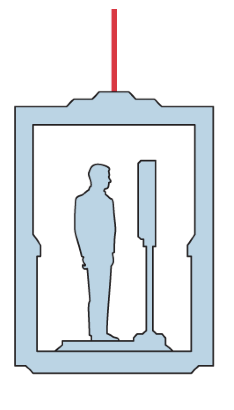
\includegraphics[width=0.25\linewidth]{./figures/e1_2.png}
  \caption{}
  \label{fig:e1_2}
\end{figure}

\bigbreak
Let $m_p = \qty{75}{kg}$ denote the mass of the person and $m = \qty{750}{kg}$ denote the entire mass of the system. Also let $F_c = \qty{8300}{N}$ denote the force in the cable. Newton's second law on the entire system gives
\[ 
m \ddot{d} = F_c - mg \implies \ddot{d} = \frac{F_c - mg}{m}
.\]
For the person inside the elevator using Newton's second law gives
\[ 
  m_p \ddot{d} = F_R - m_p g \implies F_R = m_p \ddot{d} + m_p g
\]
where $F_R$ is the reactant force the scale exerts on the person (i.e. the force the person exerts on the scale). Substituting in the previous expression for $\ddot{d}$ we get
\begin{align*}
  F_R &= m_p \left( \ddot{d} + g \right) \\
  &= m_p \left( \frac{F_c - mg}{m} + g \right) \\
  &= m_p \left( \frac{F_c}{m} \right) \\
  &= \frac{m_p F_c}{m} \\
  &= \frac{\qty{75}{kg} \cdot \qty{8300}{N}}{\qty{750}{kg}} \\
  &= \qty{830}{N} 
.\end{align*}
Therefore the scale will show a reading of \qty{830}{N}.
